\documentclass[uct_visualisation_thesis.tex]{subfiles}

\section{Instalacja}
\subsection{Wymagania sprzętowe}
W celu wykorzystania możliwości, które daje prezentowany system, należy uruchomić go na komputerze, który spełnia wymienione poniżej wymagania sprzętowe.

\begin{enumerate}
	\item Procesor: Intel Core i5-3470 3.2 GHz / AMD FX-8350 4 GHz.
	\item Pamięć RAM: 8 GB.
	\item Karta graficzna: Nvidia GTX 660 2GB / AMD HD 7870 2 GB.
	\item Miejsce na dysku twardym: 150 MB.
	\item System operacyjny: Windows Vista / 7 SP1 / 8 / 8.1 64-Bit / 10.
\end{enumerate}

\subsection{Instrukcja instalacji Windows}
Aby zainstalować aplikację na dysku lokalnym, należy uruchomić plik instalacyjny \textit{UCTVisualisationSetup.exe}. Następnie ukaże się okno przeprowadzające użytkownika przez proces instalacji. Należy wybrać folder docelowy i kliknąć przycisk \textit{Install}. Po zakończeniu procesu można zamknąć okno instalacji, zaznaczając przedtem \textit{Run UCT Visualisation}, aby bezpośrednio po zamknięciu instalatora uruchomiła się aplikacja.\\

Zainstalowana aplikacja znajduje się w folderze wskazanym przez użytkownika podczas instalacji w katalogu \textit{UCT Visualisation}. Aby uruchomić aplikację należy w niego wejść i uruchomić plik \textit{UCT Visualisation.exe}.
Okno instalacji powinno przypominać to, ukazane na rysunku \ref{rys:instalacja}.

\begin{figure}[h!]
	\centering
	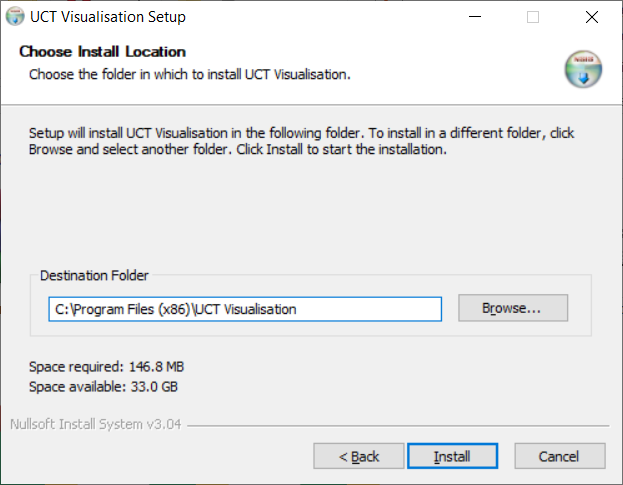
\includegraphics[width=0.7\textwidth]{instalacja}
	\caption{Okno instalacji programu}
	\label{rys:instalacja}
\end{figure}

\subsection{Instrukcja instalacji Linux}
todo
